\newcommand{\pct}[1]{\SI{#1}{\%}}
%%%%%%%%%%%%%%%%%%%%%%%%%%%%%%%%%%%%%%%%%%%%%
\subsection{$\nu_\mu$ CC Inclusive selection}
\label{ssec:NuMUCCsel:INC}
The $\nu_\mu$ CC Inclusive selection is an update from the selection described in an internal note~\cite{bib:numuccfilter}. This selection aims to be as similar as possible to the $\nu_e$ CC Inclusive selection described in \cref{sec:nueselection:inclusive}, with the ultimate goal to perform a $\nu_\mu$ constraint for a BNB electron neutrino measurement  based that $\nu_e$ selection. 

\subsubsection{$\nu_\mu$ CC inclusive signal definition}
\begin{itemize}
    \item One final state muon with a kinetic energy above \SI{20}{\MeV}.
    \item True neutrino vertex inside a fiducial volume defined with borders: \SI{10}{\cm} in $x$ and $y$ and $[ \SI{20}{\cm}, \SI{50}{\cm}]$ in $z$.
\end{itemize}
The cut on the true energy corresponds to a track length of \SI{\approx 2.5}{\cm}.

Before identifying the muon, some event level cuts are applied, as listed in Table \ref{tab:1muNp:preseInclusivel}

\begin{table}[h!]
\centering
\setlength{\tabcolsep}{10pt}
\renewcommand{\arraystretch}{1.25}
 \begin{tabular}{| c | c |} 
 \hline
 Cut goal & Cut definition \\
 \hline\hline
\multirow{5}{*}{ Cosmic rejection } & nslice = 1 \\ & slpdg= 14\\ &CosmicIP $>$ \SI{20}{\cm}\\
& topological\_score $>$ 0.1 \\ &all\_start\_contained\\
 \hline
 \end{tabular}
 \caption{\label{tab:1muNp:preseInclusivel} Preselection requirements for the $\nu_\mu$ Inclusive Selection.}
\end{table}

The next step is to identify a muon track. The requirements for muon identification are listed in Table \ref{tab:1muNp:preseInclusivelMuon}

\begin{table}[h!]
\centering
\setlength{\tabcolsep}{10pt}
\renewcommand{\arraystretch}{1.25}
 \begin{tabular}{| c | c |} 
 \hline
 Cut goal & Cut definition \\
 \hline\hline
\multirow{5}{*}{ Muon Identification } & 
trk\_score $>$ 0.8 \\ &
trk\_len $>$ \SI{10}{\cm} \\ &
trk\_llr\_pid\_score $>$ 0.2\\ &
pfp\_generation = 2  \\ &
trk\_distance $<$ \SI{4}{\cm}\\
 \hline
 \end{tabular}
 \caption{\label{tab:1muNp:preseInclusivelMuon} Muon identification requirements for the $\nu_\mu$ Inclusive Selection.}
\end{table}

At this point, the number of muon candidate tracks in signal events is:
\begin{comment}
\begin{itemize}
    \item \textit{slpdg = 14}
    \item \textit{CosmicIP} $>$ \SI{20}{\cm}
    \item \textit{topological\_score $>$ 0.1}
    \item \textit{all\_start\_contained}
\end{itemize} 

The next step is to identify a muon track.
\paragraph{Muon candidate identification} 
\begin{itemize}
    \item \textit{trk\_score $>$ 0.8}
    \item \textit{trk\_len} $>$ \SI{10}{\cm}
    \item \textit{trk\_llr\_pid\_score $>$ 0.2}
    \item \textit{pfp\_generation = 2}
    \item \textit{trk\_distance} $<$ \SI{4}{\cm}
\end{itemize}
At this point, the amount of muon candidate tracks in signal events is:
\end{comment}

\begin{itemize}
    \item 0 (10\%), the event gets rejected.
    \item 1 (70\%), the event gets selected.
    \item 2 (18\%) or $>2$ (2\%), the particle with t   he highest \textit{trk\_llr\_pid\_score} is picked as muon and the event is selected.
\end{itemize}

The cut on the reconstructed length corresponds to a muon kinetic energy of \SI{\approx 47}{\MeV} or a muon momentum of \SI{0.11}{GeV/c}. Therefore, this selection has a lower neutrino energy threshold of \SI{\approx 153}{\MeV}, and efficiency plots will be shown in a range from \SIrange{0.15}{1.65}{\GeV}.
The distribution of the topological score and the track muon likelihood after applying all cuts except these two is given in \cref{fig:numu:topo_pid}.


\begin{figure}[htb]
    \centering
    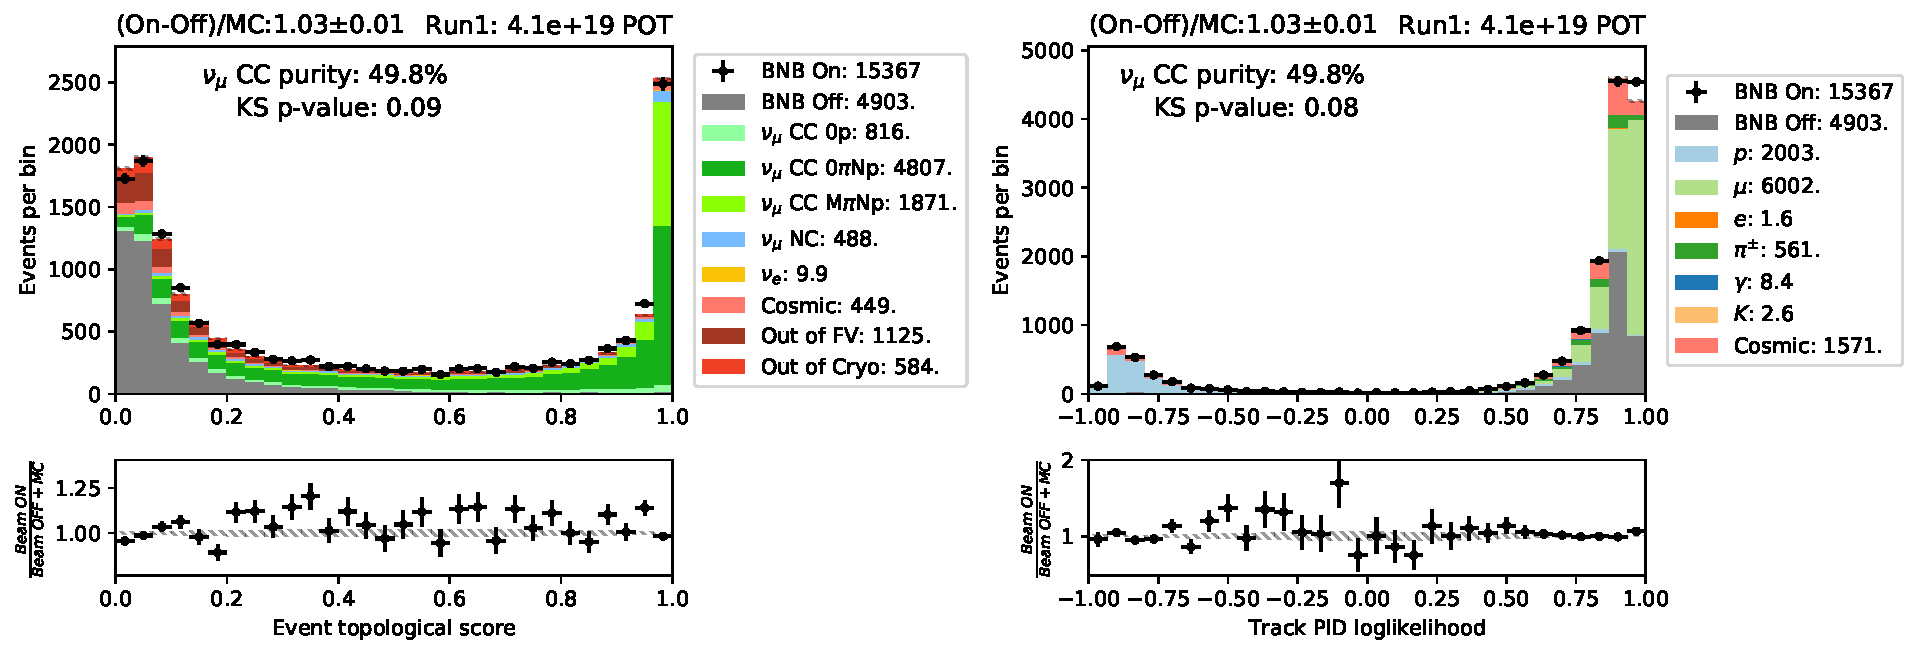
\includegraphics[width=\textwidth]{NuMuCCsel/Images/run1/numu_pret_run1.pdf}
    \caption{Topological score and track PID likelihood distributions after all other cuts are applied in the $\nu_\mu$ CC inclusive selection.}
    \label{fig:numu:topo_pid}
\end{figure}



\subsubsection{Event selection performance}

\begin{figure}[htb]
\centering
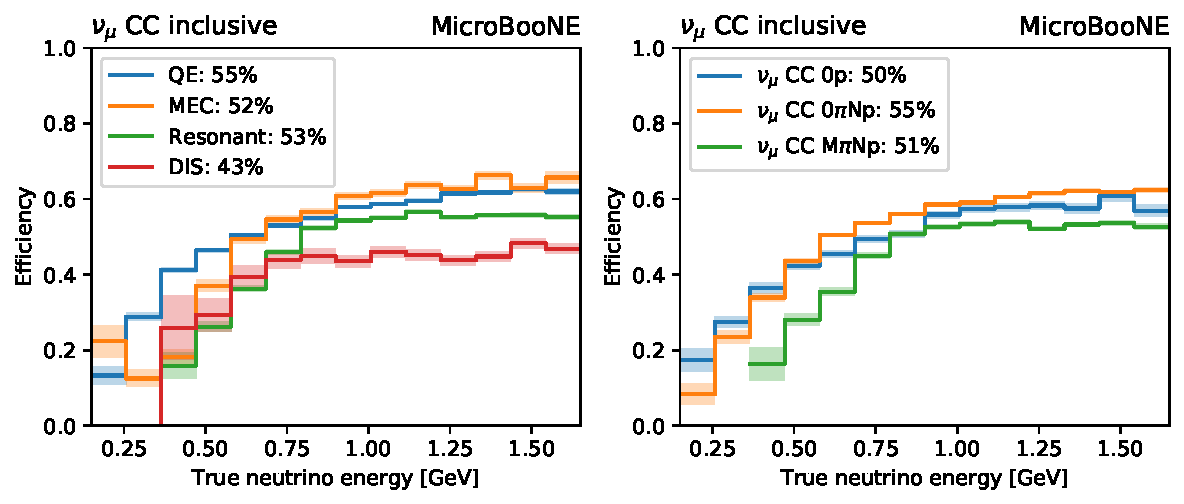
\includegraphics[width=0.65\textwidth]{Inclusive/Images/efficiency_inclusive.pdf}
\caption[Efficiency of the inclusive \numucc selection for different interaction modes and channels]{Efficiency of the inclusive \numucc selection for different interaction modes (left) and channels (right) in function of the simulated neutrino energy. The range of the $x$-axis \SIrange{0.15}{1.65}{\GeV}. The overall efficiency is \pct{53.4+-0.1}.}
\label{fig:efficiency_inclusive}
\end{figure}

\cref{fig:efficiency_inclusive} shows the efficiency in function of the true neutrino energy;  the integrated  efficiency over all energies for all signal categories is \pct{51.1}. It can be seen that the selection is truly inclusive in both interaction type and final states. non-zero efficiencies are reached from \SI{150}{\MeV} and the efficiency flattens out at \SI{\approx 700}{\MeV}. The overall purity of the selection is 64.4\% with the in-time cosmic activity as dominant background. In 94.7\% of the events, the track identified as muon is backtracked to the muon correctly. Most mis-identification cases correspond to charged pions (3.6\%). Because this selection contains both contained and uncontained events, multiple coulomb scattering is used to measure the muon momentum. Data/MC comparisons are excluded from this note due to space restrictions. 
 
\subsubsection{High purity selection}
When using the Run3 open data, we can use the CRT to achieve  a higher purity. Nonetheless, exiting muon tracks might trigger the CRT veto as well, therefore the higher purity selection includes both containment and CRT veto. The additional cuts are:
\begin{itemize}
    \item[-] \texttt{all\_end\_contained}
    \item[-] \texttt{CRT Veto} != 1 or \texttt{crthitpe} $<$ 100
    \item[-] \texttt{closestNuCosmicDist} $>$ \SI{5}{\cm}
\end{itemize}
Due to the fact that most $\nu_\mu$ CC inclusive events are not contained, the efficiency drops to 20.2\%, see \cref{fig:efficiency_contained}. Note that the denominator here still contains both contained and uncontained events to enable comparison with the previous section. At the very lowest neutrino energies, below \SI{\approx 400}{\MeV}, the efficiency is only slightly reduced. The overall purity goes up to \SI{76.4}{\%}. 

\begin{figure}[htb]
\centering
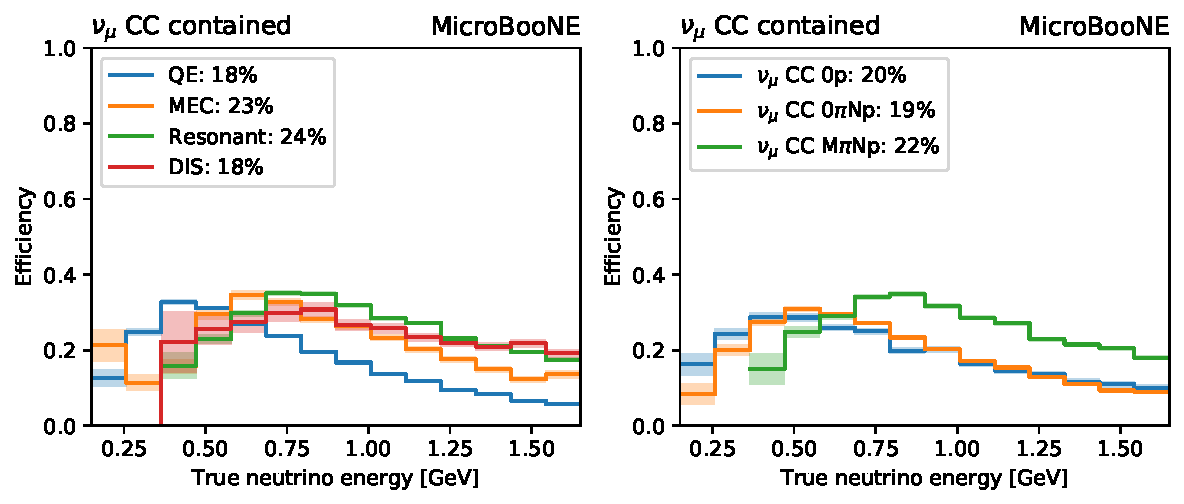
\includegraphics[width=0.65\textwidth]{Inclusive/Images/efficiency_contained.pdf}
\caption[Efficiency of the contained \numucc selection for different interaction modes and channels]{Efficiency of the contained \numucc selection for different interaction modes (left) and channels (right) in function of the simulated neutrino energy. The range of the $x$-axis \SIrange{0.15}{1.65}{\GeV}. The overall efficiency is \pct{20.2+-0.1}.}
\label{fig:efficiency_contained}
\end{figure}

\subsubsection{Lepton kinematic in the high purity selection}
\cref{fig:final_numu:reso} shows the resolution of the reconstructed lepton kinematics.
The corresponding data/MC distributions are given in \cref{fig:final_numu:datamc}. It can be seen that the flux+GENIE combined systematic uncertainties range between \SIlist{25;40}{\%}. These variables will be used to constraint the systematics in the \nuecc channel. 

\begin{figure}[htb] 
\begin{center}
    \begin{subfigure}{\textwidth}
    \centering
    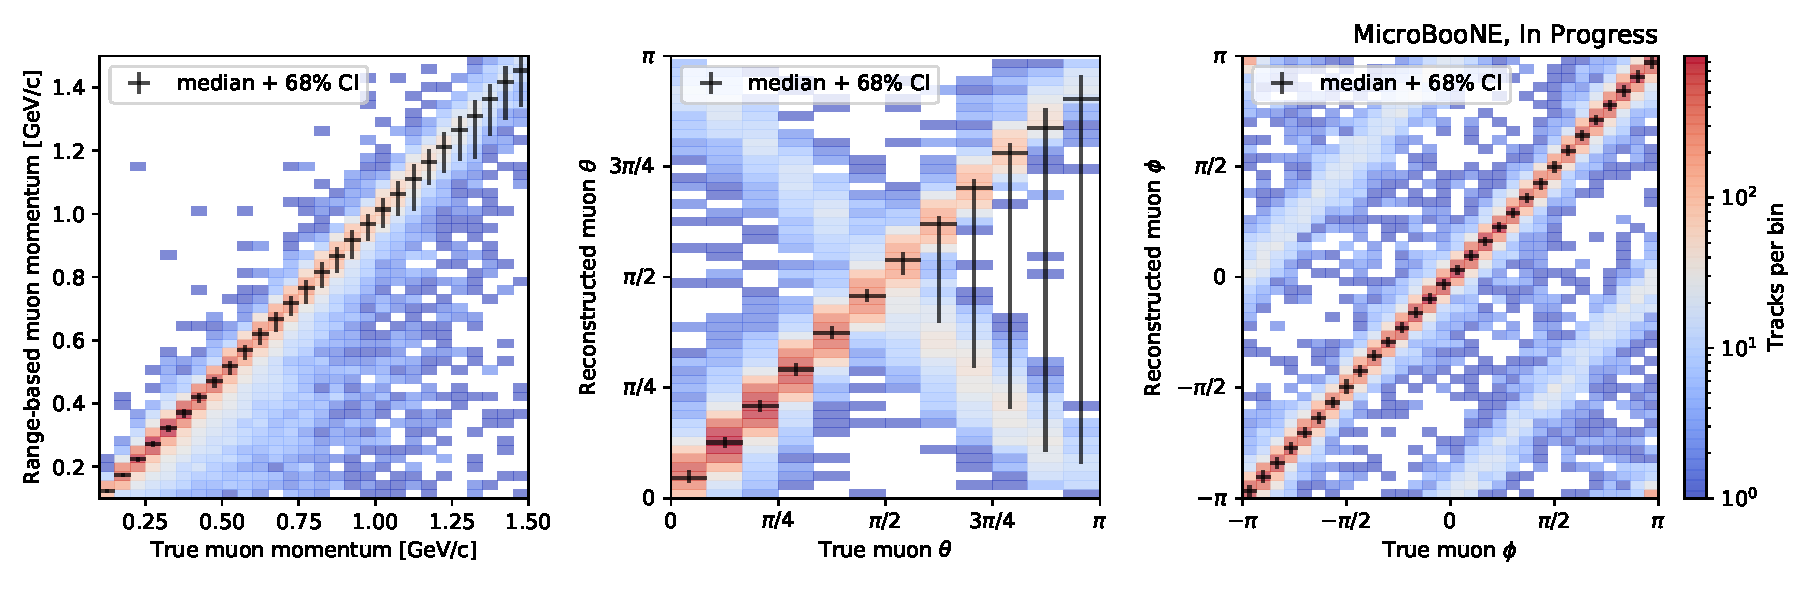
\includegraphics[width=0.9\textwidth]{Inclusive/Images/thesis_muon_resolution.pdf}
    \caption{\label{fig:final_numu:reso} Resolution in the contained \numucc selection for the muon momentum (left), muon $\theta$ (middle) and muon $\phi$ (right). The colour scale for the \textit{2D} histograms is logarithmic. In black, the median and \pct{68} confidence interval are given, binned in the true muon kinematics. For all three muon kinematics, the most probable value has as bias at the $\order{\pct{1}}$ level. The muon momentum resolution is related tot the track length. For short tracks, this is below \pct{3}, for longer tracks, that have a higher probability to enter unresponsive regions, this increases to $\order{\pct{5}}$. The middle and right plot show off-diagonal components related to reverse reconstructed muon tracks. When excluding these cases the resolution in $\theta$ is $\order{\pct{2}}$ and $\order{\pct{3}}$ for $\phi$.\\}
    \end{subfigure}
    \begin{subfigure}{\textwidth}
    \centering
    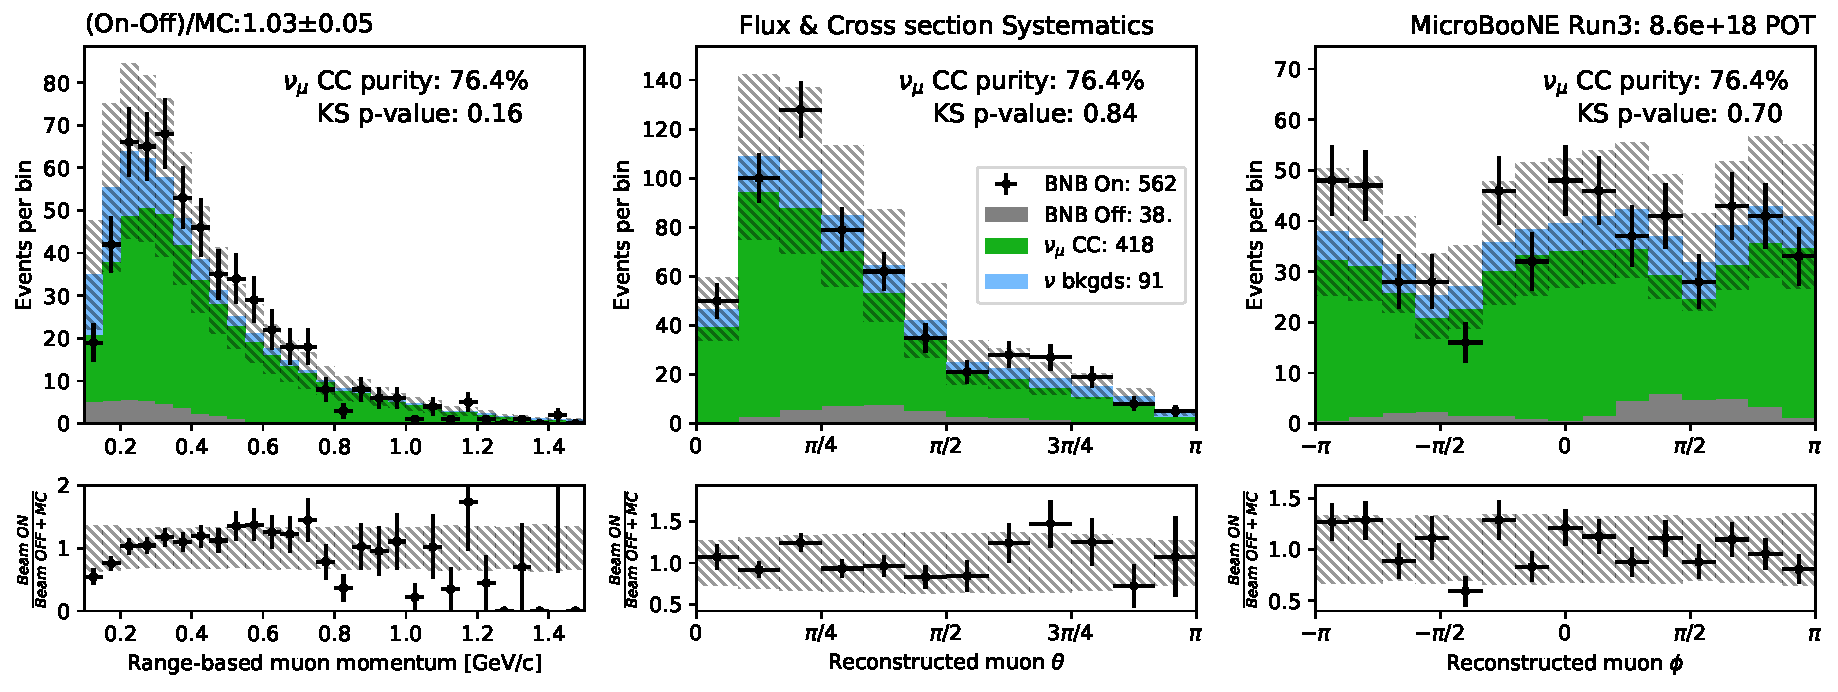
\includegraphics[width=0.88\textwidth]{Inclusive/Images/thesis_muon_kinematics_run3.pdf}
    \caption{\label{fig:final_numu:datamc} Momentum (left) and directional angles $\theta$ (middle) and $\phi$ (right) of the \numucc muon candidate. In blue, the neutrino related backgrounds are grouped into one category. The error bars on the data are Poissonian. The errors on the prediction are the flux+GENIE combined systematic uncertainties. The fractional magnitude of the systematic uncertainties ranges between \SIlist{25;40}{\%}.}
    \end{subfigure}
\caption[Lepton kinematics for the \numucc channel. Both resolution and data/MC comparisons are shown]{\label{fig:final_numu} Lepton kinematics for the \numucc channel. Both resolution (a) and Data/MC comparisons (b) are shown.}
\end{center}
\end{figure}

\clearpage